% id: 0525
% book: RPM 기하 · 05 벡터의 연산
% section: 서술형 주관식
% figure: crop:fig-0525.png
% answer: $-3$
% answer_source: 답지
% variant_level: 0 (원본 전사)
% 이 파일은 build.mjs 가 items.json 에서 만든다. 고칠 때는 items.json 을 고친다.
\smash{\raisebox{1.5mm}{\dmkichul{RPM 기하 0525번 · 83쪽}}}
\noindent\begin{minipage}[t]{0.58\linewidth}\vspace{0pt}\raggedright 오른쪽 그림과 같이 두 개의 합동인 정육각형이 한 변을 공유하고 있다. $\overrightarrow{\mathrm{OP}}=\vec{p}$, $\overrightarrow{\mathrm{OQ}}=\vec{q}$라 할 때, $\overrightarrow{\mathrm{OR}}=m\vec{p}+n\vec{q}$이다. 실수 $m$, $n$에 대하여 $mn$의 값을 구하시오.\end{minipage}\hfill\begin{minipage}[t]{0.4\linewidth}\vspace{0pt}\centering \setlength{\dmfigw}{102.3pt}\ifdim\dmfigw>\linewidth\setlength{\dmfigw}{\linewidth}\fi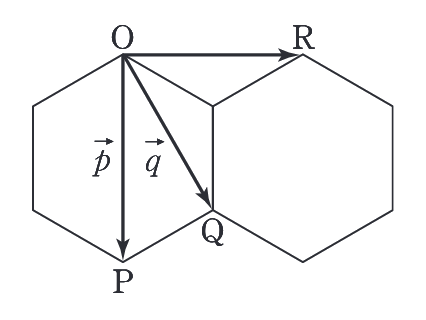
\includegraphics[width=\dmfigw]{figures/fig-0525.png}\end{minipage}\par
